\documentclass[xetex,serif]{beamer}
%\usepackage[driver=xetex,a4paper,left=35mm,right=35mm,top=30mm,bottom=40mm]{geometry} % propper margins on a4 paper
%\usepackage{url}
%\usepackage[hidelinks]{hyperref} % make contents and references clickable in pdf
\usepackage[english]{babel}
\usepackage[english]{isodate} \isodate%
\usepackage[absolute,overlay]{textpos}
\usepackage{graphicx} % include images
\usepackage{pgfplots}
\graphicspath{{graphics/}}

\usepackage{fontspec} % allows custom fonts
\setmainfont[BoldFont=Source Sans Pro Bold,AutoFakeSlant=0.3]{Source Serif Pro}
\setmonofont{Source Code Pro}

\usetheme{default}
\usecolortheme{crane}

\beamertemplatenavigationsymbolsempty

\title{Design and implementation of the\\Meta Casanova 3 compiler back-end}
\author{Douwe van Gijn}
\date{2016-06-29}

\begin{document}
\begin{frame}
\titlepage

\end{frame}\begin{frame}\frametitle{Introduction}
\begin{itemize}
    \item Games are difficult $\longrightarrow$ Casanova language
    \item Compilers are difficult $\longrightarrow$ Meta Casanova language
    \item Compilers in two parts
    \begin{enumerate}
        \item Front-end: parse and typecheck
        \item Back-end: generate executables
    \end{enumerate}
\end{itemize}

\end{frame}\begin{frame}\frametitle{Contents}
\begin{itemize}
    \item Introduction
    \item Research Question
    \item Sub-questions
    \item Results
    \item Conclusions
    \item Demo
\end{itemize}

\end{frame}\begin{frame}\frametitle{Research question}
\textit{How to implement a transformation from typechecked Meta Casanova from the front-end, to executable code within the timeframe of the internship?}

\end{frame}\begin{frame}\frametitle{Requirements}
\begin{itemize}
    \item The correctness requirement
    \item The .NET requirement
    \item The multiplatform requirement
    \item The performance requirement
\end{itemize}

\end{frame}\begin{frame}[t]\frametitle{Sub-questions}
\begin{itemize}
    \item 7 sub-questions
    \item Each answer implements parts of the back-end
    %\item The language question
    %\item The interface question
    %\item The IR question
    %\item The codegen question
    %\item The mangle question
    %\item The validation question
    %\item The debug question
\end{itemize}
\begin{textblock*}{0.75\paperwidth}(0.125\paperwidth,6cm)\includegraphics[width=0.75\paperwidth]{overview}\end{textblock*}

\end{frame}\begin{frame}[t]\frametitle{The language question}
\textit{In what language should the code generator produce its output?}
\begin{itemize}
    \item Researched lots of langages
    \item Two feasable: C\# or F\#
    \item Implemented both code-models
    \item C\# won out
    \begin{itemize}
        \item more readable
        \item easier to generate
        \item faster
    \end{itemize}
\end{itemize}
\begin{textblock*}{0.75\paperwidth}(0.125\paperwidth,6cm)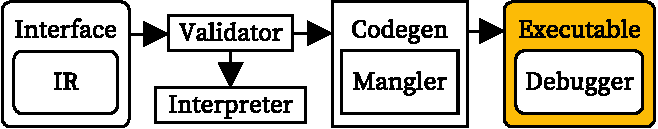
\includegraphics[width=0.75\paperwidth]{overview_language}\end{textblock*}

\end{frame}\begin{frame}[t]\frametitle{The interface question}
\textit{What should the interface be between the front-end and the back-end?}
\begin{itemize}
    \item Contains all inputs of back-end 
    \item Validator validates invariants
\end{itemize}
\begin{textblock*}{0.75\paperwidth}(0.125\paperwidth,6cm)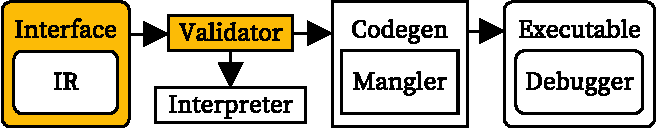
\includegraphics[width=0.75\paperwidth]{overview_interface}\end{textblock*}

\end{frame}\begin{frame}[t]\frametitle{The IR question}
\textit{What should the Intermediate Representation of the function be?}
\begin{itemize}
    \item Instruction set for MC
    \item Minimal and orthogonal
    \item Only 6 base instructions
\end{itemize}
\begin{textblock*}{0.75\paperwidth}(0.125\paperwidth,6cm)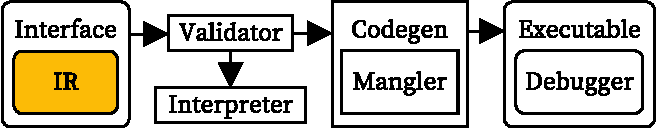
\includegraphics[width=0.75\paperwidth]{overview_ir}\end{textblock*}

\end{frame}\begin{frame}[t]\frametitle{The codegen question}
\textit{How does the interface map to the output language?}
\begin{itemize}
    \item Generates program structure
    \item Translates IR to C\# instructions
\end{itemize}
\begin{textblock*}{0.75\paperwidth}(0.125\paperwidth,6cm)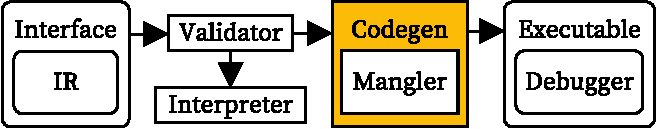
\includegraphics[width=0.75\paperwidth]{overview_codegen}\end{textblock*}

\end{frame}\begin{frame}[t]\frametitle{The mangle question}
\textit{How to generate names so they comply with the output language?}
\begin{itemize}
    \item MC identifiers $\longrightarrow$ C\# identifiers
    \item No name conflicts
\end{itemize}
\begin{textblock*}{0.75\paperwidth}(0.125\paperwidth,6cm)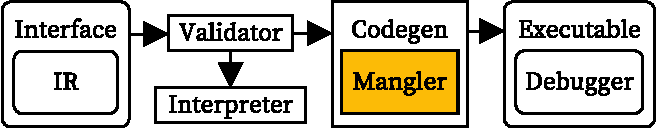
\includegraphics[width=0.75\paperwidth]{overview_mangler}\end{textblock*}

\end{frame}\begin{frame}[t]\frametitle{The validation question}
\textit{How to validate the code-gen?}
\begin{itemize}
    \item Built an interpreter!
    \item Compare results of interpreter and codegen
\end{itemize}
\begin{textblock*}{0.75\paperwidth}(0.125\paperwidth,6cm)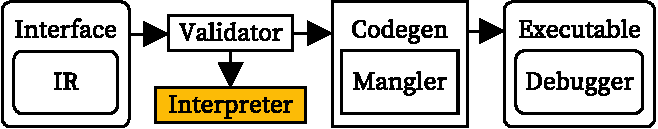
\includegraphics[width=0.75\paperwidth]{overview_validation}\end{textblock*}

\end{frame}\begin{frame}[t]\frametitle{The debug question}
\textit{How to validate the test-programs?}
\begin{itemize}
    \item Interactive debugger
    \item Embedded in executable
\end{itemize}
\begin{textblock*}{0.75\paperwidth}(0.125\paperwidth,6cm)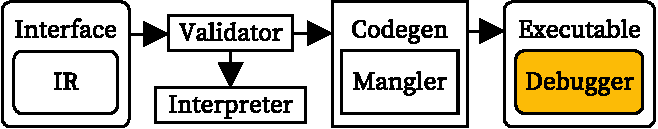
\includegraphics[width=0.75\paperwidth]{overview_debugger}\end{textblock*}

\end{frame}\begin{frame}\frametitle{Results}
\begin{itemize}
    \item The correctness requirement
    \item The .NET requirement
    \item The multiplatform requirement
    \item The performance requirement
\end{itemize}

\end{frame}\begin{frame}\frametitle{The correctness \& .NET requirement}
    Test programs

\end{frame}\begin{frame}\frametitle{The multiplatform requirement}
    Microsoft .NET Compiler for windows

    Mono everywhere else

\end{frame}\begin{frame}\frametitle{The performance requirement}
\begin{itemize}
    \item Length of list
    \item Inductive list in MC
    \item Library list in Python
    \item 1000 lists of 1 000 000 elements
\end{itemize}

\end{frame}\begin{frame}\frametitle{The performance requirement}
\begin{tikzpicture}
\begin{axis}[
        symbolic x coords={Min, Avg, Max},
        xtick=data,
	x tick label style={},
        ylabel=time/element ($\mu$s),
	enlargelimits=0.2,
        ymajorgrids=true,
        axis x line*=bottom,
        axis y line*=left,
	legend style={at={(1.1,0.5)},
	anchor=west,legend columns=1},
	ybar,
]
\addplot[black,fill=gray]   coordinates {(Min,39.00) (Avg,41.95) (Max,52.86)};
\addplot[black,fill=craneorange] coordinates {(Min,22.82) (Avg,36.30) (Max,49.79)};
\legend{Python,MC}
\end{axis}
\end{tikzpicture}

\end{frame}\begin{frame}\frametitle{Conclusion}
\begin{itemize}
    \item All requirements are met
    \item Working back-end within the allocated time
    \item Demo time!
\end{itemize}

\end{frame}\begin{frame}\frametitle{Defence}
    \begin{center}
        {%
        \setlength{\fboxsep}{0pt}%
        \fbox{\includegraphics[width=0.75\paperwidth]{defence}}%
        }%
    \end{center}

\end{frame}
\end{document}
